\documentclass[11pt,a4paper]{jarticle}
\usepackage[dvipdfmx]{graphicx}
\usepackage{url}

\renewcommand{\baselinestretch}{1.05} 
\marginparwidth=0cm
\topmargin=-1cm
\headheight=0.3cm
\headsep=0.7cm
\oddsidemargin=0cm
\evensidemargin=0cm
%\textwidth=43zw
\textwidth=15.92cm
%\textheight=43.3\baselineskip
\baselineskip = 0.5744cm
\textheight=43\baselineskip

\itemsep=0.05\baselineskip
\parsep=0pt
\topsep=0.01\baselineskip
\partopsep=0pt
\listparindent=0zw

%% header and footer
\usepackage{fancyhdr}
\pagestyle{fancy}
\lhead{2016年度 春学期授業}
\chead{インタラクティブ・アート実習}
\rhead{担当教員: 松下 光範}
\cfoot{\thepage}
\renewcommand{\headrulewidth}{0pt}
\renewcommand{\footrulewidth}{0pt}

\usepackage{ascmac}
\usepackage{listings,jlisting}
\usepackage{color}
\definecolor{OliveGreen}{cmyk}{0.64,0,0.95,0.40}
\definecolor{colFunc}{rgb}{1,0.07,0.54}
\definecolor{CadetBlue}{cmyk}{0.62,0.57,0.23,0}
\definecolor{Brown}{cmyk}{0,0.81,1,0.60}
\definecolor{colID}{rgb}{0.63,0.44,0}
\definecolor{rulesepcolor}{gray}{0.666}
\lstset{
  language=Java,%プログラミング言語によって変える。
  basicstyle={\ttfamily\small},
  keywordstyle={\color{OliveGreen}},
  %[2][3]はプログラミング言語によってあったり、なかったり
  keywordstyle={[2]\color{colFunc}},
  keywordstyle={[3]\color{CadetBlue}},%
  commentstyle={\color{Brown}},
  %identifierstyle={\color{colID}},
  stringstyle=\color{blue},
  tabsize=2,
  %frame=trBL,
  %numbers=left,
  numberstyle={\ttfamily\small},
  breaklines=true,%折り返し
  %backgroundcolor={\color[gray]{.95}},
  framexleftmargin=0mm,
  frame=single,
  rulesepcolor=\color{rulesepcolor},
  captionpos=b
}


%%%%%%%%%%%%%%%%%%%%%%%%%%%%%%%%%%%%%%%%%%%%%%%%%%%%%%%%%%%%%%%%
\begin{document}

% title
\section*{\LARGE{第6講 応用編: 赤外線センサを用いて距離を測る}}
\section{本実習の目標}
\begin{itemize}
 \item 赤外線センサを用いて、センサと物体との距離を測定する。
\end{itemize}

%%%%%%%%%%%%%%%%%%%%%%%%%%%%%%%%%%%%%%%%%%%%%%%%%%%%%%%%%%%%%%%%

\section{赤外線センサを用いて距離を測る}
物体との距離を非接触で測定するための方式には「超音波方式」と「赤外線方式」があります。
赤外線センサは、(その名の通り)赤外線を用いて距離を測定しています。
超音波センサは、物体から人体まで幅広いものの距離を検出することができます。

今回利用する赤外線センサは、大体 10cm 〜 80cm までの距離を測定することができます。
赤外線センサは、外光による影響を受けやすいため、使用する環境によっては注意する必要があります。
赤外線センサよりも、もう少し長い距離を測定したい場合は、超音波センサを使うと良いでしょう。

% 赤外線センサの図と配線の説明を入れる

\begin{itembox}[l]{注意!}
 赤外線センサは、とてもデリケートで配線の向きを間違えただけでも破損してしまいます。
 PC に接続する前に配線が正しいかどうか、もう一度確認すること!
\end{itembox}

\subsection*{回路}
\begin{figure}[h!]
 \begin{minipage}{0.5\columnwidth}
  \centering
  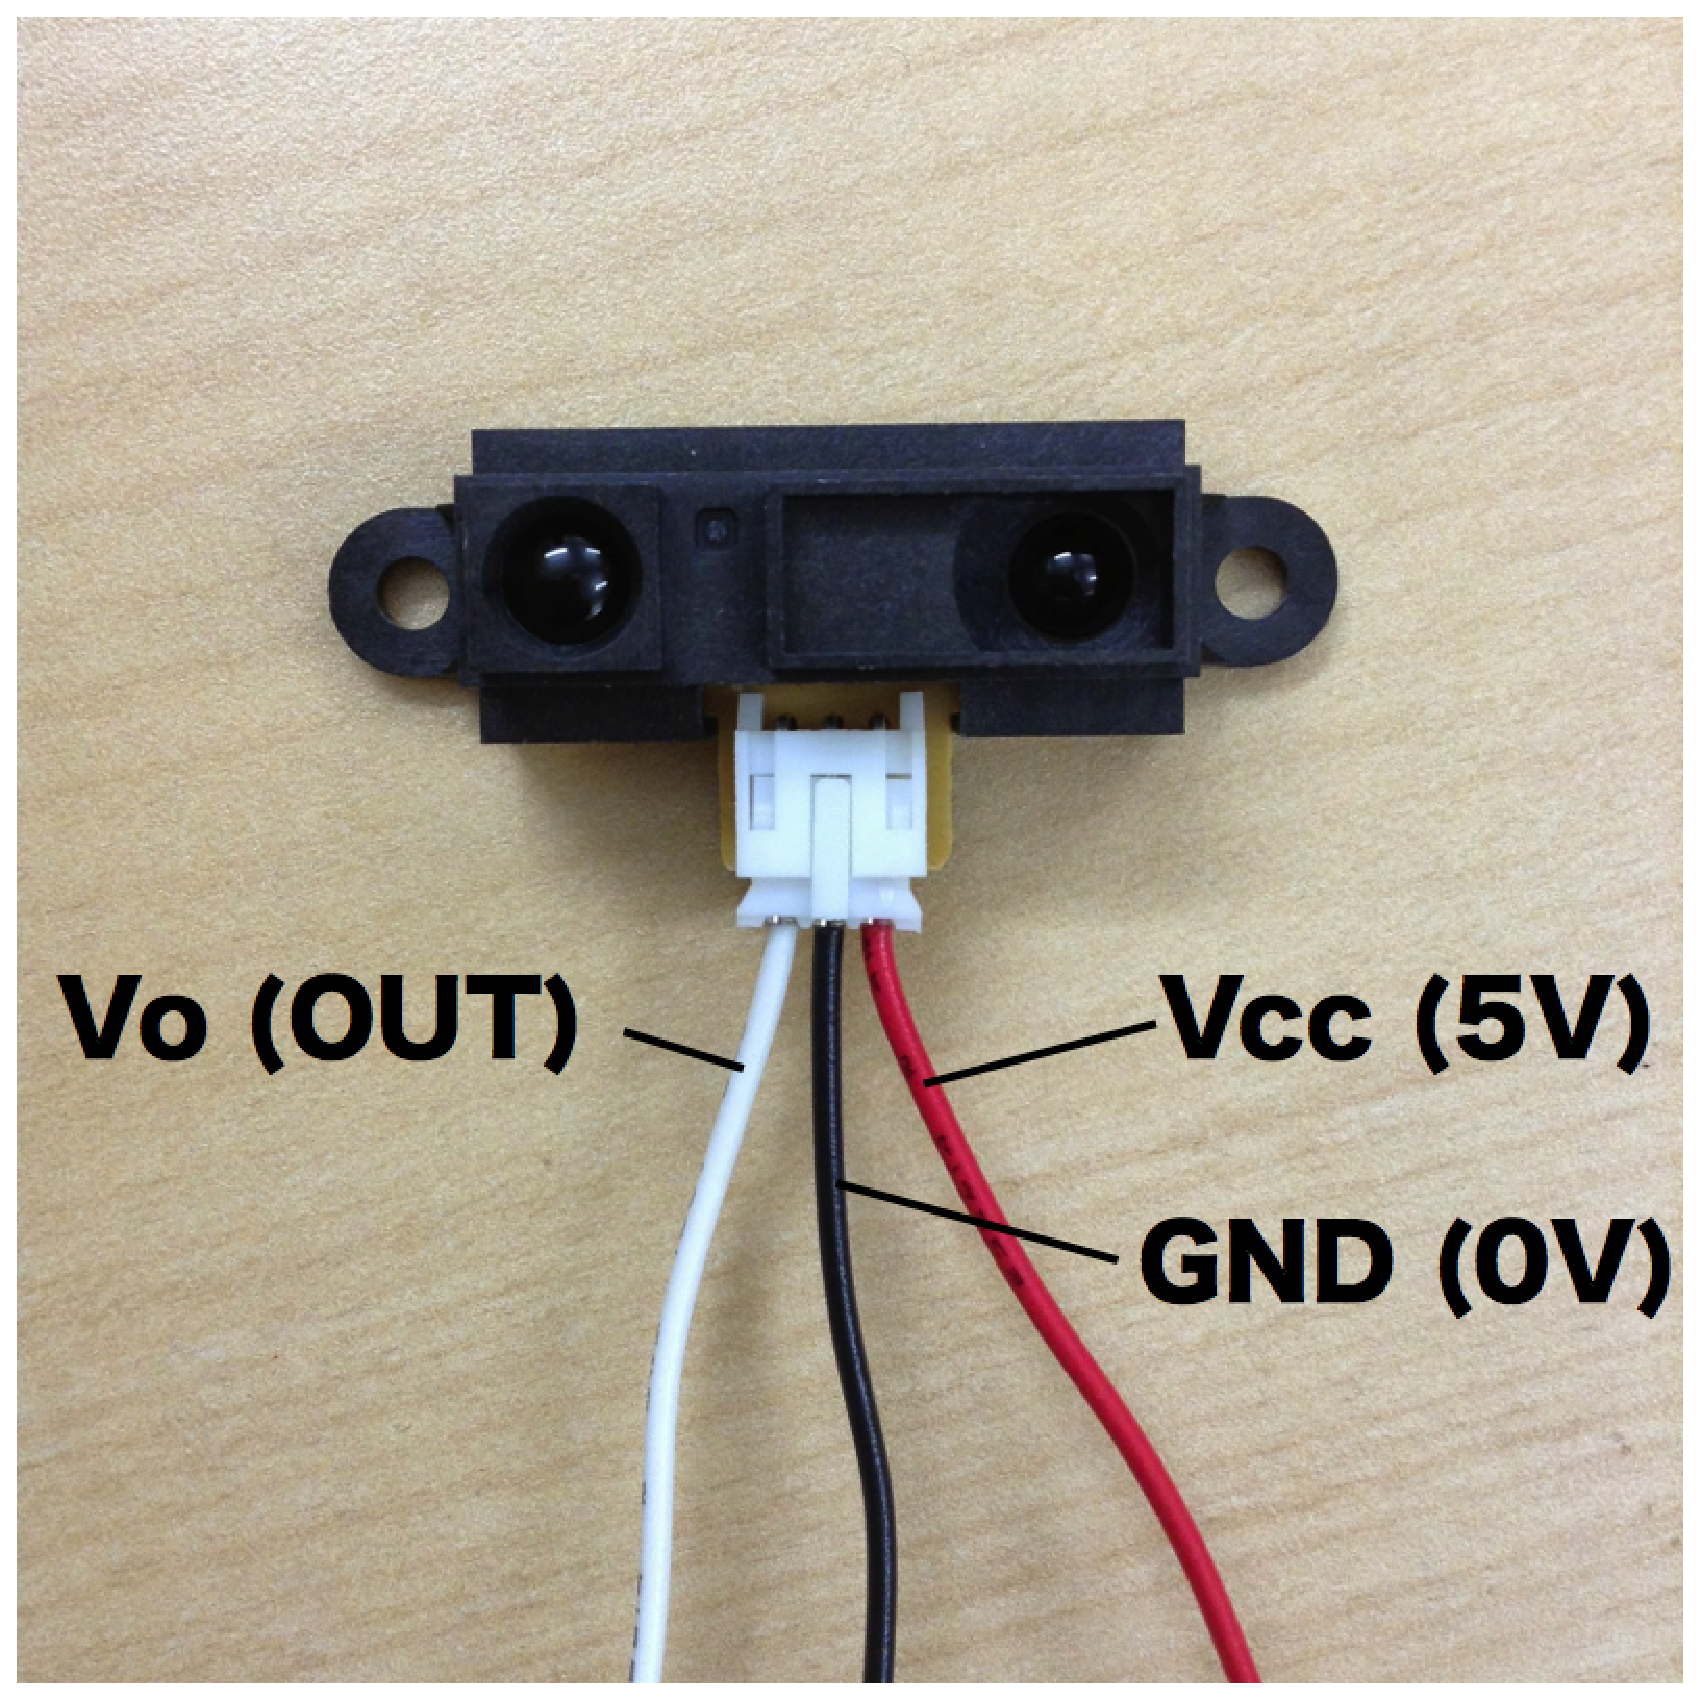
\includegraphics[width=0.7\columnwidth]{img/ir_sensor.eps}
  \begin{center}
   \textbf{赤外線センサ}
  \end{center}
 \end{minipage}
 \begin{minipage}{0.5\columnwidth}
  \centering
  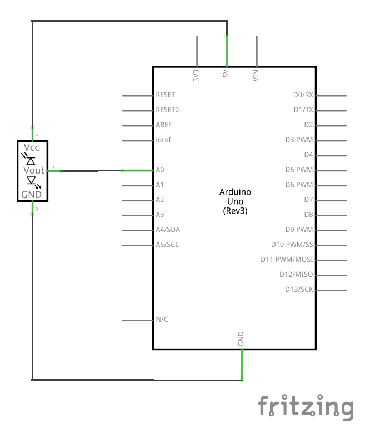
\includegraphics[width=\columnwidth]{img/infrared_proximity_circuit.eps}
  \begin{center}
   \textbf{赤外線センサを用いた回路図}
  \end{center}
 \end{minipage}
\end{figure}


\subsection*{プログラム}
光センサを曲げセンサに置き換えたときのように、プログラムは同じものが使えます。

\section{センサの値を実際の距離にマッピングする}
距離センサと後述する map 関数を組み合わせると、電子ものさしを作ることができます。

\subsection*{準備}
距離センサの値を取得して、数値がどのように変化するのか観察してみましょう。
また、センサの値が実際の距離とどのように対応付いているのをメモしておいてください。

\subsection*{map関数}
Processing には map 関数という機能が用意されています。
\begin{lstlisting}
 float y = map(x, xBegin, xEnd, yBegin, yEnd);
\end{lstlisting}
map 関数は非常に便利なので覚えておくとよいでしょう。

map 関数は x を範囲 xMin〜xMax から別の範囲 yMin〜yMax へ変換する関数です。
map 関数を利用して、センサの値を実際の距離の計測値に変換してみましょう。

\begin{lstlisting}
 void draw() {
   background(255);

   int val = arduino.analogRead(sensorPin);

   // 例、
   // 距離が
   // 10cmのとき、センサの値が768で
   // 80cmのとき、センサの値が255の場合
   float distance = map(val, 768, 255, 10, 80);

   textFont(font, 32);
   fill(0);
   text(" val: " + val, 32, 32);
   text("distance: " + distance, 32, 64);
 }
\end{lstlisting}

\end{document}